\documentclass[1p]{elsarticle_modified}
%\bibliographystyle{elsarticle-num}

%\usepackage[colorlinks]{hyperref}
%\usepackage{abbrmath_seonhwa} %\Abb, \Ascr, \Acal ,\Abf, \Afrak
\usepackage{amsfonts}
\usepackage{amssymb}
\usepackage{amsmath}
\usepackage{amsthm}
\usepackage{scalefnt}
\usepackage{amsbsy}
\usepackage{kotex}
\usepackage{caption}
\usepackage{subfig}
\usepackage{color}
\usepackage{graphicx}
\usepackage{xcolor} %% white, black, red, green, blue, cyan, magenta, yellow
\usepackage{float}
\usepackage{setspace}
\usepackage{hyperref}

\usepackage{tikz}
\usetikzlibrary{arrows}

\usepackage{multirow}
\usepackage{array} % fixed length table
\usepackage{hhline}

%%%%%%%%%%%%%%%%%%%%%
\makeatletter
\renewcommand*\env@matrix[1][\arraystretch]{%
	\edef\arraystretch{#1}%
	\hskip -\arraycolsep
	\let\@ifnextchar\new@ifnextchar
	\array{*\c@MaxMatrixCols c}}
\makeatother %https://tex.stackexchange.com/questions/14071/how-can-i-increase-the-line-spacing-in-a-matrix
%%%%%%%%%%%%%%%

\usepackage[normalem]{ulem}

\newcommand{\msout}[1]{\ifmmode\text{\sout{\ensuremath{#1}}}\else\sout{#1}\fi}
%SOURCE: \msout is \stkout macro in https://tex.stackexchange.com/questions/20609/strikeout-in-math-mode

\newcommand{\cancel}[1]{
	\ifmmode
	{\color{red}\msout{#1}}
	\else
	{\color{red}\sout{#1}}
	\fi
}

\newcommand{\add}[1]{
	{\color{blue}\uwave{#1}}
}

\newcommand{\replace}[2]{
	\ifmmode
	{\color{red}\msout{#1}}{\color{blue}\uwave{#2}}
	\else
	{\color{red}\sout{#1}}{\color{blue}\uwave{#2}}
	\fi
}

\newcommand{\Sol}{\mathcal{S}} %segment
\newcommand{\D}{D} %diagram
\newcommand{\A}{\mathcal{A}} %arc


%%%%%%%%%%%%%%%%%%%%%%%%%%%%%5 test

\def\sl{\operatorname{\textup{SL}}(2,\Cbb)}
\def\psl{\operatorname{\textup{PSL}}(2,\Cbb)}
\def\quan{\mkern 1mu \triangleright \mkern 1mu}

\theoremstyle{definition}
\newtheorem{thm}{Theorem}[section]
\newtheorem{prop}[thm]{Proposition}
\newtheorem{lem}[thm]{Lemma}
\newtheorem{ques}[thm]{Question}
\newtheorem{cor}[thm]{Corollary}
\newtheorem{defn}[thm]{Definition}
\newtheorem{exam}[thm]{Example}
\newtheorem{rmk}[thm]{Remark}
\newtheorem{alg}[thm]{Algorithm}

\newcommand{\I}{\sqrt{-1}}
\begin{document}

%\begin{frontmatter}
%
%\title{Boundary parabolic representations of knots up to 8 crossings}
%
%%% Group authors per affiliation:
%\author{Yunhi Cho} 
%\address{Department of Mathematics, University of Seoul, Seoul, Korea}
%\ead{yhcho@uos.ac.kr}
%
%
%\author{Seonhwa Kim} %\fnref{s_kim}}
%\address{Center for Geometry and Physics, Institute for Basic Science, Pohang, 37673, Korea}
%\ead{ryeona17@ibs.re.kr}
%
%\author{Hyuk Kim}
%\address{Department of Mathematical Sciences, Seoul National University, Seoul 08826, Korea}
%\ead{hyukkim@snu.ac.kr}
%
%\author{Seokbeom Yoon}
%\address{Department of Mathematical Sciences, Seoul National University, Seoul, 08826,  Korea}
%\ead{sbyoon15@snu.ac.kr}
%
%\begin{abstract}
%We find all boundary parabolic representation of knots up to 8 crossings.
%
%\end{abstract}
%\begin{keyword}
%    \MSC[2010] 57M25 
%\end{keyword}
%
%\end{frontmatter}

%\linenumbers
%\tableofcontents
%
\newcommand\colored[1]{\textcolor{white}{\rule[-0.35ex]{0.8em}{1.4ex}}\kern-0.8em\color{red} #1}%
%\newcommand\colored[1]{\textcolor{white}{ #1}\kern-2.17ex	\textcolor{white}{ #1}\kern-1.81ex	\textcolor{white}{ #1}\kern-2.15ex\color{red}#1	}

{\Large $\underline{12a_{0134}~(K12a_{0134})}$}

\setlength{\tabcolsep}{10pt}
\renewcommand{\arraystretch}{1.6}
\vspace{1cm}\begin{tabular}{m{100pt}>{\centering\arraybackslash}m{274pt}}
\multirow{5}{120pt}{
	\centering
	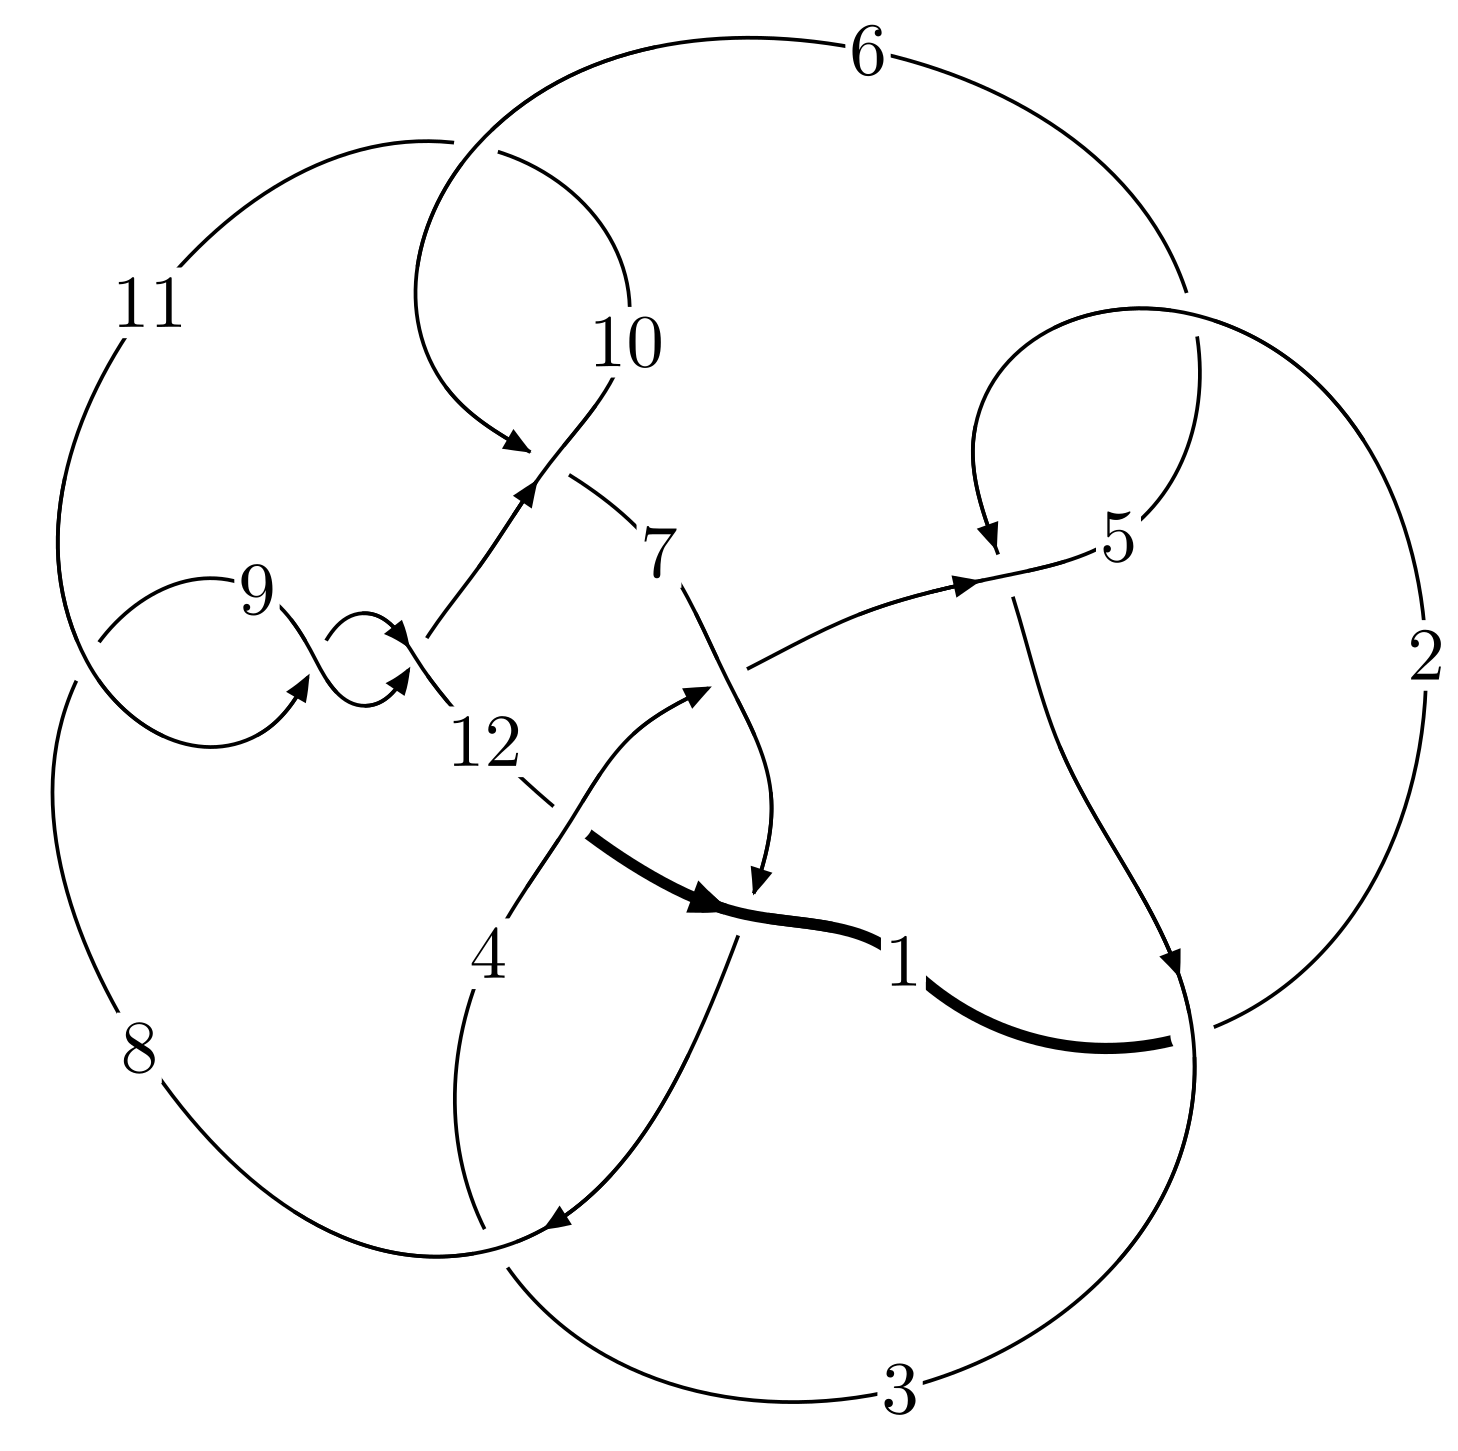
\includegraphics[width=112pt]{../../../GIT/diagram.site/Diagrams/png/935_12a_0134.png}\\
\ \ \ A knot diagram\footnotemark}&
\allowdisplaybreaks
\textbf{Linearized knot diagam} \\
\cline{2-2}
 &
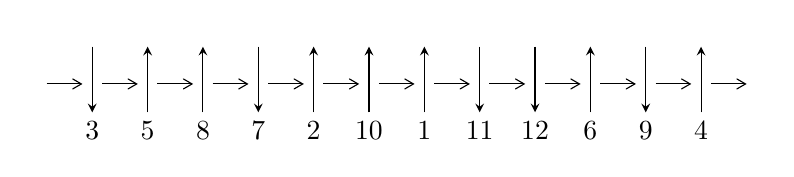
\begin{tikzpicture}[x=20pt, y=17pt]
	% nodes
	\node (C0) at (0, 0) {};
	\node (C1) at (1, 0) {};
	\node (C1U) at (1, +1) {};
	\node (C1D) at (1, -1) {3};

	\node (C2) at (2, 0) {};
	\node (C2U) at (2, +1) {};
	\node (C2D) at (2, -1) {5};

	\node (C3) at (3, 0) {};
	\node (C3U) at (3, +1) {};
	\node (C3D) at (3, -1) {8};

	\node (C4) at (4, 0) {};
	\node (C4U) at (4, +1) {};
	\node (C4D) at (4, -1) {7};

	\node (C5) at (5, 0) {};
	\node (C5U) at (5, +1) {};
	\node (C5D) at (5, -1) {2};

	\node (C6) at (6, 0) {};
	\node (C6U) at (6, +1) {};
	\node (C6D) at (6, -1) {10};

	\node (C7) at (7, 0) {};
	\node (C7U) at (7, +1) {};
	\node (C7D) at (7, -1) {1};

	\node (C8) at (8, 0) {};
	\node (C8U) at (8, +1) {};
	\node (C8D) at (8, -1) {11};

	\node (C9) at (9, 0) {};
	\node (C9U) at (9, +1) {};
	\node (C9D) at (9, -1) {12};

	\node (C10) at (10, 0) {};
	\node (C10U) at (10, +1) {};
	\node (C10D) at (10, -1) {6};

	\node (C11) at (11, 0) {};
	\node (C11U) at (11, +1) {};
	\node (C11D) at (11, -1) {9};

	\node (C12) at (12, 0) {};
	\node (C12U) at (12, +1) {};
	\node (C12D) at (12, -1) {4};
	\node (C13) at (13, 0) {};

	% arrows
	\draw[->,>={angle 60}]
	(C0) edge (C1) (C1) edge (C2) (C2) edge (C3) (C3) edge (C4) (C4) edge (C5) (C5) edge (C6) (C6) edge (C7) (C7) edge (C8) (C8) edge (C9) (C9) edge (C10) (C10) edge (C11) (C11) edge (C12) (C12) edge (C13) ;	\draw[->,>=stealth]
	(C1U) edge (C1D) (C2D) edge (C2U) (C3D) edge (C3U) (C4U) edge (C4D) (C5D) edge (C5U) (C6D) edge (C6U) (C7D) edge (C7U) (C8U) edge (C8D) (C9U) edge (C9D) (C10D) edge (C10U) (C11U) edge (C11D) (C12D) edge (C12U) ;
	\end{tikzpicture} \\
\hhline{~~} \\& 
\textbf{Solving Sequence} \\ \cline{2-2} 
 &
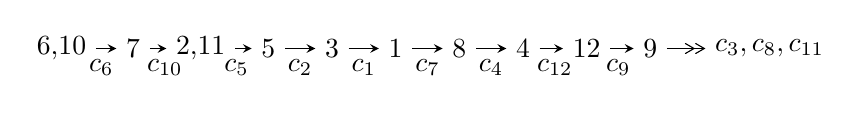
\begin{tikzpicture}[x=23pt, y=7pt]
	% node
	\node (A0) at (-1/8, 0) {6,10};
	\node (A1) at (1, 0) {7};
	\node (A2) at (33/16, 0) {2,11};
	\node (A3) at (25/8, 0) {5};
	\node (A4) at (33/8, 0) {3};
	\node (A5) at (41/8, 0) {1};
	\node (A6) at (49/8, 0) {8};
	\node (A7) at (57/8, 0) {4};
	\node (A8) at (65/8, 0) {12};
	\node (A9) at (73/8, 0) {9};
	\node (C1) at (1/2, -1) {$c_{6}$};
	\node (C2) at (3/2, -1) {$c_{10}$};
	\node (C3) at (21/8, -1) {$c_{5}$};
	\node (C4) at (29/8, -1) {$c_{2}$};
	\node (C5) at (37/8, -1) {$c_{1}$};
	\node (C6) at (45/8, -1) {$c_{7}$};
	\node (C7) at (53/8, -1) {$c_{4}$};
	\node (C8) at (61/8, -1) {$c_{12}$};
	\node (C9) at (69/8, -1) {$c_{9}$};
	\node (A10) at (11, 0) {$c_{3},c_{8},c_{11}$};

	% edge
	\draw[->,>=stealth]	
	(A0) edge (A1) (A1) edge (A2) (A2) edge (A3) (A3) edge (A4) (A4) edge (A5) (A5) edge (A6) (A6) edge (A7) (A7) edge (A8) (A8) edge (A9) ;
	\draw[->>,>={angle 60}]	
	(A9) edge (A10);
\end{tikzpicture} \\ 

\end{tabular} \\

\footnotetext{
The image of knot diagram is generated by the software ``\textbf{Draw programme}" developed by Andrew Bartholomew(\url{http://www.layer8.co.uk/maths/draw/index.htm\#Running-draw}), where we modified some parts for our purpose(\url{https://github.com/CATsTAILs/LinksPainter}).
}\phantom \\ \newline 
\centering \textbf{Ideals for irreducible components\footnotemark of $X_{\text{par}}$} 
 
\begin{align*}
I^u_{1}&=\langle 
-1.86227\times10^{495} u^{118}-4.68618\times10^{495} u^{117}+\cdots+1.43467\times10^{497} b-3.00236\times10^{498},\\
\phantom{I^u_{1}}&\phantom{= \langle  }4.78619\times10^{497} u^{118}-1.23447\times10^{498} u^{117}+\cdots+4.47045\times10^{499} a-1.58926\times10^{501},\\
\phantom{I^u_{1}}&\phantom{= \langle  }u^{119}+u^{118}+\cdots+4096 u+512\rangle \\
\\
I^v_{1}&=\langle 
a,\;59103 v^8-362866 v^7+\cdots+178147 b+551223,\;v^9-5 v^8+10 v^7- v^5-37 v^4+7 v^3-12 v^2+v-1\rangle \\
\end{align*}
\raggedright * 2 irreducible components of $\dim_{\mathbb{C}}=0$, with total 128 representations.\\
\footnotetext{All coefficients of polynomials are rational numbers. But the coefficients are sometimes approximated in decimal forms when there is not enough margin.}
\newpage
\renewcommand{\arraystretch}{1}
\centering \section*{I. $I^u_{1}= \langle -1.86\times10^{495} u^{118}-4.69\times10^{495} u^{117}+\cdots+1.43\times10^{497} b-3.00\times10^{498},\;4.79\times10^{497} u^{118}-1.23\times10^{498} u^{117}+\cdots+4.47\times10^{499} a-1.59\times10^{501},\;u^{119}+u^{118}+\cdots+4096 u+512 \rangle$}
\flushleft \textbf{(i) Arc colorings}\\
\begin{tabular}{m{7pt} m{180pt} m{7pt} m{180pt} }
\flushright $a_{6}=$&$\begin{pmatrix}1\\0\end{pmatrix}$ \\
\flushright $a_{10}=$&$\begin{pmatrix}0\\u\end{pmatrix}$ \\
\flushright $a_{7}=$&$\begin{pmatrix}1\\- u^2\end{pmatrix}$ \\
\flushright $a_{2}=$&$\begin{pmatrix}-0.0107063 u^{118}+0.0276140 u^{117}+\cdots+265.664 u+35.5505\\0.0129804 u^{118}+0.0326637 u^{117}+\cdots+174.370 u+20.9271\end{pmatrix}$ \\
\flushright $a_{11}=$&$\begin{pmatrix}u\\u\end{pmatrix}$ \\
\flushright $a_{5}=$&$\begin{pmatrix}-0.0499003 u^{118}-0.0301250 u^{117}+\cdots+96.3323 u+17.6475\\-0.0248375 u^{118}-0.0192909 u^{117}+\cdots+27.4367 u+5.81828\end{pmatrix}$ \\
\flushright $a_{3}=$&$\begin{pmatrix}-0.0668403 u^{118}-0.0545125 u^{117}+\cdots-0.779841 u+6.91602\\-0.0284835 u^{118}-0.0271884 u^{117}+\cdots-88.5312 u-7.25798\end{pmatrix}$ \\
\flushright $a_{1}=$&$\begin{pmatrix}0.0132150 u^{118}-0.0126096 u^{117}+\cdots-186.921 u-26.5168\\-0.0237768 u^{118}-0.0244099 u^{117}+\cdots-41.8929 u-2.43633\end{pmatrix}$ \\
\flushright $a_{8}=$&$\begin{pmatrix}0.00385505 u^{118}-0.00206836 u^{117}+\cdots-60.8198 u-8.57415\\0.0354571 u^{118}+0.00289238 u^{117}+\cdots-230.820 u-34.3222\end{pmatrix}$ \\
\flushright $a_{4}=$&$\begin{pmatrix}-0.0508154 u^{118}-0.0358733 u^{117}+\cdots+68.3183 u+13.3408\\-0.0261492 u^{118}-0.0238212 u^{117}+\cdots+7.17127 u+3.34367\end{pmatrix}$ \\
\flushright $a_{12}=$&$\begin{pmatrix}-0.0316021 u^{118}-0.00496074 u^{117}+\cdots+170.000 u+25.7481\\-0.0478118 u^{118}-0.00189380 u^{117}+\cdots+323.763 u+47.9626\end{pmatrix}$ \\
\flushright $a_{9}=$&$\begin{pmatrix}0.0162097 u^{118}-0.00306695 u^{117}+\cdots-153.762 u-22.2145\\0.0478118 u^{118}+0.00189380 u^{117}+\cdots-323.763 u-47.9626\end{pmatrix}$\\&\end{tabular}
\flushleft \textbf{(ii) Obstruction class $= -1$}\\~\\
\flushleft \textbf{(iii) Cusp Shapes $= 0.155199 u^{118}+0.132157 u^{117}+\cdots+22.3469 u-16.4864$}\\~\\
\newpage\renewcommand{\arraystretch}{1}
\flushleft \textbf{(iv) u-Polynomials at the component}\newline \\
\begin{tabular}{m{50pt}|m{274pt}}
Crossings & \hspace{64pt}u-Polynomials at each crossing \\
\hline $$\begin{aligned}c_{1}\end{aligned}$$&$\begin{aligned}
&u^{119}+48 u^{118}+\cdots-10 u-1
\end{aligned}$\\
\hline $$\begin{aligned}c_{2},c_{5}\end{aligned}$$&$\begin{aligned}
&u^{119}+2 u^{118}+\cdots-10 u-1
\end{aligned}$\\
\hline $$\begin{aligned}c_{3}\end{aligned}$$&$\begin{aligned}
&u^{119}-2 u^{118}+\cdots+8762 u-1327
\end{aligned}$\\
\hline $$\begin{aligned}c_{4}\end{aligned}$$&$\begin{aligned}
&u^{119}-6 u^{118}+\cdots-3844 u-1441
\end{aligned}$\\
\hline $$\begin{aligned}c_{6},c_{10}\end{aligned}$$&$\begin{aligned}
&u^{119}- u^{118}+\cdots+4096 u-512
\end{aligned}$\\
\hline $$\begin{aligned}c_{7}\end{aligned}$$&$\begin{aligned}
&u^{119}+10 u^{118}+\cdots-2 u-1
\end{aligned}$\\
\hline $$\begin{aligned}c_{8},c_{9},c_{11}\end{aligned}$$&$\begin{aligned}
&u^{119}-10 u^{118}+\cdots+14 u-1
\end{aligned}$\\
\hline $$\begin{aligned}c_{12}\end{aligned}$$&$\begin{aligned}
&u^{119}+12 u^{118}+\cdots-2 u-1
\end{aligned}$\\
\hline
\end{tabular}\\~\\
\newpage\renewcommand{\arraystretch}{1}
\flushleft \textbf{(v) Riley Polynomials at the component}\newline \\
\begin{tabular}{m{50pt}|m{274pt}}
Crossings & \hspace{64pt}Riley Polynomials at each crossing \\
\hline $$\begin{aligned}c_{1}\end{aligned}$$&$\begin{aligned}
&y^{119}+48 y^{118}+\cdots-1922 y-1
\end{aligned}$\\
\hline $$\begin{aligned}c_{2},c_{5}\end{aligned}$$&$\begin{aligned}
&y^{119}+48 y^{118}+\cdots-10 y-1
\end{aligned}$\\
\hline $$\begin{aligned}c_{3}\end{aligned}$$&$\begin{aligned}
&y^{119}-132 y^{118}+\cdots+73112778 y-1760929
\end{aligned}$\\
\hline $$\begin{aligned}c_{4}\end{aligned}$$&$\begin{aligned}
&y^{119}-108 y^{118}+\cdots-880963674 y-2076481
\end{aligned}$\\
\hline $$\begin{aligned}c_{6},c_{10}\end{aligned}$$&$\begin{aligned}
&y^{119}+57 y^{118}+\cdots-1572864 y-262144
\end{aligned}$\\
\hline $$\begin{aligned}c_{7}\end{aligned}$$&$\begin{aligned}
&y^{119}-12 y^{118}+\cdots+10 y-1
\end{aligned}$\\
\hline $$\begin{aligned}c_{8},c_{9},c_{11}\end{aligned}$$&$\begin{aligned}
&y^{119}-108 y^{118}+\cdots-162 y-1
\end{aligned}$\\
\hline $$\begin{aligned}c_{12}\end{aligned}$$&$\begin{aligned}
&y^{119}+100 y^{117}+\cdots-10 y-1
\end{aligned}$\\
\hline
\end{tabular}\\~\\
\newpage\flushleft \textbf{(vi) Complex Volumes and Cusp Shapes}
$$\begin{array}{c|c|c}  
\text{Solutions to }I^u_{1}& \I (\text{vol} + \sqrt{-1}CS) & \text{Cusp shape}\\
 \hline 
\begin{aligned}
u &= \phantom{-}0.526423 + 0.832737 I \\
a &= -0.379040 + 0.949735 I \\
b &= \phantom{-}0.955538 + 0.601021 I\end{aligned}
 & \phantom{-}2.70873 + 3.86349 I & \phantom{-0.000000 } 0 \\ \hline\begin{aligned}
u &= \phantom{-}0.526423 - 0.832737 I \\
a &= -0.379040 - 0.949735 I \\
b &= \phantom{-}0.955538 - 0.601021 I\end{aligned}
 & \phantom{-}2.70873 - 3.86349 I & \phantom{-0.000000 } 0 \\ \hline\begin{aligned}
u &= \phantom{-}0.921604 + 0.339981 I \\
a &= \phantom{-}0.599719 + 0.536043 I \\
b &= -0.675300 + 1.052770 I\end{aligned}
 & \phantom{-}2.91318 - 8.94395 I & \phantom{-0.000000 } 0 \\ \hline\begin{aligned}
u &= \phantom{-}0.921604 - 0.339981 I \\
a &= \phantom{-}0.599719 - 0.536043 I \\
b &= -0.675300 - 1.052770 I\end{aligned}
 & \phantom{-}2.91318 + 8.94395 I & \phantom{-0.000000 } 0 \\ \hline\begin{aligned}
u &= -0.497653 + 0.822885 I \\
a &= \phantom{-}0.555826 + 0.047006 I \\
b &= \phantom{-}0.115814 - 0.219568 I\end{aligned}
 & \phantom{-}0.04303 - 1.98692 I & \phantom{-0.000000 } 0 \\ \hline\begin{aligned}
u &= -0.497653 - 0.822885 I \\
a &= \phantom{-}0.555826 - 0.047006 I \\
b &= \phantom{-}0.115814 + 0.219568 I\end{aligned}
 & \phantom{-}0.04303 + 1.98692 I & \phantom{-0.000000 } 0 \\ \hline\begin{aligned}
u &= \phantom{-}0.848144 + 0.441248 I \\
a &= \phantom{-}0.653233 - 0.314441 I \\
b &= -0.822990 - 0.578925 I\end{aligned}
 & \phantom{-}4.34687 - 3.34050 I & \phantom{-0.000000 } 0 \\ \hline\begin{aligned}
u &= \phantom{-}0.848144 - 0.441248 I \\
a &= \phantom{-}0.653233 + 0.314441 I \\
b &= -0.822990 + 0.578925 I\end{aligned}
 & \phantom{-}4.34687 + 3.34050 I & \phantom{-0.000000 } 0 \\ \hline\begin{aligned}
u &= -0.395311 + 0.868690 I \\
a &= -4.40337 - 2.54920 I \\
b &= \phantom{-}0.525263 - 0.898450 I\end{aligned}
 & -0.25612 - 3.85842 I & \phantom{-0.000000 } 0 \\ \hline\begin{aligned}
u &= -0.395311 - 0.868690 I \\
a &= -4.40337 + 2.54920 I \\
b &= \phantom{-}0.525263 + 0.898450 I\end{aligned}
 & -0.25612 + 3.85842 I & \phantom{-0.000000 } 0\\
 \hline 
 \end{array}$$\newpage$$\begin{array}{c|c|c}  
\text{Solutions to }I^u_{1}& \I (\text{vol} + \sqrt{-1}CS) & \text{Cusp shape}\\
 \hline 
\begin{aligned}
u &= -1.000340 + 0.308388 I \\
a &= \phantom{-}0.686162 + 0.562362 I \\
b &= -0.625987 + 0.939108 I\end{aligned}
 & \phantom{-}2.82823 - 5.08911 I & \phantom{-0.000000 } 0 \\ \hline\begin{aligned}
u &= -1.000340 - 0.308388 I \\
a &= \phantom{-}0.686162 - 0.562362 I \\
b &= -0.625987 - 0.939108 I\end{aligned}
 & \phantom{-}2.82823 + 5.08911 I & \phantom{-0.000000 } 0 \\ \hline\begin{aligned}
u &= \phantom{-}0.486144 + 0.934868 I \\
a &= -1.21381 + 2.09573 I \\
b &= \phantom{-}0.687854 + 1.176020 I\end{aligned}
 & \phantom{-}0.50738 + 6.41058 I & \phantom{-0.000000 } 0 \\ \hline\begin{aligned}
u &= \phantom{-}0.486144 - 0.934868 I \\
a &= -1.21381 - 2.09573 I \\
b &= \phantom{-}0.687854 - 1.176020 I\end{aligned}
 & \phantom{-}0.50738 - 6.41058 I & \phantom{-0.000000 } 0 \\ \hline\begin{aligned}
u &= -0.100723 + 1.062340 I \\
a &= \phantom{-}0.08824 - 2.61983 I \\
b &= -0.072083 - 1.177180 I\end{aligned}
 & -5.55472 - 1.58319 I & \phantom{-0.000000 } 0 \\ \hline\begin{aligned}
u &= -0.100723 - 1.062340 I \\
a &= \phantom{-}0.08824 + 2.61983 I \\
b &= -0.072083 + 1.177180 I\end{aligned}
 & -5.55472 + 1.58319 I & \phantom{-0.000000 } 0 \\ \hline\begin{aligned}
u &= -0.868718 + 0.318232 I \\
a &= -0.208382 - 0.342220 I \\
b &= \phantom{-}0.625738 + 1.148730 I\end{aligned}
 & -2.17047 + 4.66203 I & \phantom{-0.000000 } 0 \\ \hline\begin{aligned}
u &= -0.868718 - 0.318232 I \\
a &= -0.208382 + 0.342220 I \\
b &= \phantom{-}0.625738 - 1.148730 I\end{aligned}
 & -2.17047 - 4.66203 I & \phantom{-0.000000 } 0 \\ \hline\begin{aligned}
u &= \phantom{-}0.002867 + 0.924913 I \\
a &= \phantom{-}0.529675 - 0.759000 I \\
b &= -0.224374 - 0.203815 I\end{aligned}
 & -1.31680 - 1.56421 I & \phantom{-0.000000 } 0 \\ \hline\begin{aligned}
u &= \phantom{-}0.002867 - 0.924913 I \\
a &= \phantom{-}0.529675 + 0.759000 I \\
b &= -0.224374 + 0.203815 I\end{aligned}
 & -1.31680 + 1.56421 I & \phantom{-0.000000 } 0\\
 \hline 
 \end{array}$$\newpage$$\begin{array}{c|c|c}  
\text{Solutions to }I^u_{1}& \I (\text{vol} + \sqrt{-1}CS) & \text{Cusp shape}\\
 \hline 
\begin{aligned}
u &= \phantom{-}0.535297 + 0.750461 I \\
a &= \phantom{-}0.483410 + 0.719185 I \\
b &= \phantom{-}0.939624 - 0.355644 I\end{aligned}
 & \phantom{-}2.95353 + 0.44405 I & \phantom{-0.000000 } 0 \\ \hline\begin{aligned}
u &= \phantom{-}0.535297 - 0.750461 I \\
a &= \phantom{-}0.483410 - 0.719185 I \\
b &= \phantom{-}0.939624 + 0.355644 I\end{aligned}
 & \phantom{-}2.95353 - 0.44405 I & \phantom{-0.000000 } 0 \\ \hline\begin{aligned}
u &= \phantom{-}0.843634 + 0.305336 I \\
a &= \phantom{-}1.053140 + 0.212736 I \\
b &= -0.146729 - 0.103716 I\end{aligned}
 & -2.62882 - 0.46286 I & \phantom{-0.000000 } 0 \\ \hline\begin{aligned}
u &= \phantom{-}0.843634 - 0.305336 I \\
a &= \phantom{-}1.053140 - 0.212736 I \\
b &= -0.146729 + 0.103716 I\end{aligned}
 & -2.62882 + 0.46286 I & \phantom{-0.000000 } 0 \\ \hline\begin{aligned}
u &= -0.417757 + 0.773293 I \\
a &= -0.71113 - 2.74755 I \\
b &= \phantom{-}0.520079 + 0.812541 I\end{aligned}
 & \phantom{-}0.027445 + 0.372128 I & \phantom{-0.000000 } 0 \\ \hline\begin{aligned}
u &= -0.417757 - 0.773293 I \\
a &= -0.71113 + 2.74755 I \\
b &= \phantom{-}0.520079 - 0.812541 I\end{aligned}
 & \phantom{-}0.027445 - 0.372128 I & \phantom{-0.000000 } 0 \\ \hline\begin{aligned}
u &= -0.859101 + 0.154610 I \\
a &= \phantom{-}0.637106 - 0.427319 I \\
b &= -0.664918 - 0.727137 I\end{aligned}
 & \phantom{-}3.48096 - 0.06555 I & \phantom{-0.000000 } 0 \\ \hline\begin{aligned}
u &= -0.859101 - 0.154610 I \\
a &= \phantom{-}0.637106 + 0.427319 I \\
b &= -0.664918 + 0.727137 I\end{aligned}
 & \phantom{-}3.48096 + 0.06555 I & \phantom{-0.000000 } 0 \\ \hline\begin{aligned}
u &= -0.209029 + 0.820458 I \\
a &= \phantom{-}1.24444 + 4.72940 I \\
b &= \phantom{-}0.431964 + 0.872764 I\end{aligned}
 & -0.797814 + 0.550209 I & \phantom{-}12.54758 + 0. I\phantom{ +0.000000I} \\ \hline\begin{aligned}
u &= -0.209029 - 0.820458 I \\
a &= \phantom{-}1.24444 - 4.72940 I \\
b &= \phantom{-}0.431964 - 0.872764 I\end{aligned}
 & -0.797814 - 0.550209 I & \phantom{-}12.54758 + 0. I\phantom{ +0.000000I}\\
 \hline 
 \end{array}$$\newpage$$\begin{array}{c|c|c}  
\text{Solutions to }I^u_{1}& \I (\text{vol} + \sqrt{-1}CS) & \text{Cusp shape}\\
 \hline 
\begin{aligned}
u &= -1.118120 + 0.282841 I \\
a &= \phantom{-}0.571251 + 0.676237 I \\
b &= -0.036836 + 1.239910 I\end{aligned}
 & -6.98001 + 4.13299 I & \phantom{-0.000000 } 0 \\ \hline\begin{aligned}
u &= -1.118120 - 0.282841 I \\
a &= \phantom{-}0.571251 - 0.676237 I \\
b &= -0.036836 - 1.239910 I\end{aligned}
 & -6.98001 - 4.13299 I & \phantom{-0.000000 } 0 \\ \hline\begin{aligned}
u &= -0.398186 + 1.085280 I \\
a &= -0.040349 + 0.323432 I \\
b &= \phantom{-}0.921149 + 1.021620 I\end{aligned}
 & -3.27191 - 0.12438 I & \phantom{-0.000000 } 0 \\ \hline\begin{aligned}
u &= -0.398186 - 1.085280 I \\
a &= -0.040349 - 0.323432 I \\
b &= \phantom{-}0.921149 - 1.021620 I\end{aligned}
 & -3.27191 + 0.12438 I & \phantom{-0.000000 } 0 \\ \hline\begin{aligned}
u &= -0.411359 + 1.083630 I \\
a &= -0.693040 + 0.000352 I \\
b &= -0.819404 - 0.474535 I\end{aligned}
 & \phantom{-}0.08564 - 3.67293 I & \phantom{-0.000000 } 0 \\ \hline\begin{aligned}
u &= -0.411359 - 1.083630 I \\
a &= -0.693040 - 0.000352 I \\
b &= -0.819404 + 0.474535 I\end{aligned}
 & \phantom{-}0.08564 + 3.67293 I & \phantom{-0.000000 } 0 \\ \hline\begin{aligned}
u &= \phantom{-}0.819575 + 0.109814 I \\
a &= -3.51686 - 2.94234 I \\
b &= \phantom{-}0.487246 - 0.894874 I\end{aligned}
 & -2.55503 - 2.22852 I & \phantom{-}26.2651 - 22.7094 I \\ \hline\begin{aligned}
u &= \phantom{-}0.819575 - 0.109814 I \\
a &= -3.51686 + 2.94234 I \\
b &= \phantom{-}0.487246 + 0.894874 I\end{aligned}
 & -2.55503 + 2.22852 I & \phantom{-}26.2651 + 22.7094 I \\ \hline\begin{aligned}
u &= \phantom{-}0.443863 + 1.094740 I \\
a &= -0.70279 + 2.05830 I \\
b &= \phantom{-}0.010995 + 1.274440 I\end{aligned}
 & -4.33720 + 6.36777 I & \phantom{-0.000000 } 0 \\ \hline\begin{aligned}
u &= \phantom{-}0.443863 - 1.094740 I \\
a &= -0.70279 - 2.05830 I \\
b &= \phantom{-}0.010995 - 1.274440 I\end{aligned}
 & -4.33720 - 6.36777 I & \phantom{-0.000000 } 0\\
 \hline 
 \end{array}$$\newpage$$\begin{array}{c|c|c}  
\text{Solutions to }I^u_{1}& \I (\text{vol} + \sqrt{-1}CS) & \text{Cusp shape}\\
 \hline 
\begin{aligned}
u &= -0.478462 + 1.080620 I \\
a &= \phantom{-}0.235074 - 0.378978 I \\
b &= \phantom{-}1.109330 + 0.253117 I\end{aligned}
 & -1.80179 - 3.47511 I & \phantom{-0.000000 } 0 \\ \hline\begin{aligned}
u &= -0.478462 - 1.080620 I \\
a &= \phantom{-}0.235074 + 0.378978 I \\
b &= \phantom{-}1.109330 - 0.253117 I\end{aligned}
 & -1.80179 + 3.47511 I & \phantom{-0.000000 } 0 \\ \hline\begin{aligned}
u &= -0.278092 + 1.159260 I \\
a &= \phantom{-}0.28192 + 1.45729 I \\
b &= \phantom{-}0.411679 + 1.308160 I\end{aligned}
 & -6.92350 + 1.57130 I & \phantom{-0.000000 } 0 \\ \hline\begin{aligned}
u &= -0.278092 - 1.159260 I \\
a &= \phantom{-}0.28192 - 1.45729 I \\
b &= \phantom{-}0.411679 - 1.308160 I\end{aligned}
 & -6.92350 - 1.57130 I & \phantom{-0.000000 } 0 \\ \hline\begin{aligned}
u &= \phantom{-}0.482491 + 0.622840 I \\
a &= \phantom{-}0.207877 - 0.091383 I \\
b &= \phantom{-}0.755776 - 1.020320 I\end{aligned}
 & \phantom{-}1.44329 - 2.36124 I & \phantom{-}8.29903 + 4.18833 I \\ \hline\begin{aligned}
u &= \phantom{-}0.482491 - 0.622840 I \\
a &= \phantom{-}0.207877 + 0.091383 I \\
b &= \phantom{-}0.755776 + 1.020320 I\end{aligned}
 & \phantom{-}1.44329 + 2.36124 I & \phantom{-}8.29903 - 4.18833 I \\ \hline\begin{aligned}
u &= -0.667291 + 0.411587 I \\
a &= \phantom{-}0.43420 - 2.04602 I \\
b &= \phantom{-}0.820942 + 0.613116 I\end{aligned}
 & -0.08315 + 2.49375 I & \phantom{-}7.75933 - 3.67875 I \\ \hline\begin{aligned}
u &= -0.667291 - 0.411587 I \\
a &= \phantom{-}0.43420 + 2.04602 I \\
b &= \phantom{-}0.820942 - 0.613116 I\end{aligned}
 & -0.08315 - 2.49375 I & \phantom{-}7.75933 + 3.67875 I \\ \hline\begin{aligned}
u &= \phantom{-}0.490044 + 1.116310 I \\
a &= \phantom{-}0.282231 - 0.161432 I \\
b &= \phantom{-}0.420670 + 0.336969 I\end{aligned}
 & -4.94221 + 5.12424 I & \phantom{-0.000000 } 0 \\ \hline\begin{aligned}
u &= \phantom{-}0.490044 - 1.116310 I \\
a &= \phantom{-}0.282231 + 0.161432 I \\
b &= \phantom{-}0.420670 - 0.336969 I\end{aligned}
 & -4.94221 - 5.12424 I & \phantom{-0.000000 } 0\\
 \hline 
 \end{array}$$\newpage$$\begin{array}{c|c|c}  
\text{Solutions to }I^u_{1}& \I (\text{vol} + \sqrt{-1}CS) & \text{Cusp shape}\\
 \hline 
\begin{aligned}
u &= \phantom{-}0.451345 + 1.135050 I \\
a &= -0.611010 + 1.164460 I \\
b &= \phantom{-}0.590546 - 0.752125 I\end{aligned}
 & -5.11734 + 2.47956 I & \phantom{-0.000000 } 0 \\ \hline\begin{aligned}
u &= \phantom{-}0.451345 - 1.135050 I \\
a &= -0.611010 - 1.164460 I \\
b &= \phantom{-}0.590546 + 0.752125 I\end{aligned}
 & -5.11734 - 2.47956 I & \phantom{-0.000000 } 0 \\ \hline\begin{aligned}
u &= -0.529740 + 1.114830 I \\
a &= -0.360715 - 0.684753 I \\
b &= \phantom{-}1.073270 - 0.683609 I\end{aligned}
 & -2.26487 - 7.17835 I & \phantom{-0.000000 } 0 \\ \hline\begin{aligned}
u &= -0.529740 - 1.114830 I \\
a &= -0.360715 + 0.684753 I \\
b &= \phantom{-}1.073270 + 0.683609 I\end{aligned}
 & -2.26487 + 7.17835 I & \phantom{-0.000000 } 0 \\ \hline\begin{aligned}
u &= -1.141570 + 0.512721 I \\
a &= \phantom{-}0.672303 + 0.260569 I \\
b &= -0.874943 + 0.463475 I\end{aligned}
 & -0.86473 + 6.53924 I & \phantom{-0.000000 } 0 \\ \hline\begin{aligned}
u &= -1.141570 - 0.512721 I \\
a &= \phantom{-}0.672303 - 0.260569 I \\
b &= -0.874943 - 0.463475 I\end{aligned}
 & -0.86473 - 6.53924 I & \phantom{-0.000000 } 0 \\ \hline\begin{aligned}
u &= -0.399609 + 1.211290 I \\
a &= \phantom{-}0.74296 + 2.11227 I \\
b &= -0.641203 + 1.096930 I\end{aligned}
 & -1.77422 - 9.13916 I & \phantom{-0.000000 } 0 \\ \hline\begin{aligned}
u &= -0.399609 - 1.211290 I \\
a &= \phantom{-}0.74296 - 2.11227 I \\
b &= -0.641203 - 1.096930 I\end{aligned}
 & -1.77422 + 9.13916 I & \phantom{-0.000000 } 0 \\ \hline\begin{aligned}
u &= \phantom{-}0.370969 + 1.226650 I \\
a &= \phantom{-}0.06002 - 2.55757 I \\
b &= \phantom{-}0.377258 - 0.977217 I\end{aligned}
 & -6.68223 + 1.86961 I & \phantom{-0.000000 } 0 \\ \hline\begin{aligned}
u &= \phantom{-}0.370969 - 1.226650 I \\
a &= \phantom{-}0.06002 + 2.55757 I \\
b &= \phantom{-}0.377258 + 0.977217 I\end{aligned}
 & -6.68223 - 1.86961 I & \phantom{-0.000000 } 0\\
 \hline 
 \end{array}$$\newpage$$\begin{array}{c|c|c}  
\text{Solutions to }I^u_{1}& \I (\text{vol} + \sqrt{-1}CS) & \text{Cusp shape}\\
 \hline 
\begin{aligned}
u &= -0.527861 + 0.486187 I \\
a &= -0.73012 - 1.84153 I \\
b &= \phantom{-}0.751631 - 0.403800 I\end{aligned}
 & \phantom{-}0.107706 - 0.619941 I & \phantom{-}7.54549 + 5.15553 I \\ \hline\begin{aligned}
u &= -0.527861 - 0.486187 I \\
a &= -0.73012 + 1.84153 I \\
b &= \phantom{-}0.751631 + 0.403800 I\end{aligned}
 & \phantom{-}0.107706 + 0.619941 I & \phantom{-}7.54549 - 5.15553 I \\ \hline\begin{aligned}
u &= \phantom{-}0.615601 + 1.128990 I \\
a &= -0.438959 - 0.352835 I \\
b &= -0.913238 + 0.486014 I\end{aligned}
 & \phantom{-}2.23345 + 8.79850 I & \phantom{-0.000000 } 0 \\ \hline\begin{aligned}
u &= \phantom{-}0.615601 - 1.128990 I \\
a &= -0.438959 + 0.352835 I \\
b &= -0.913238 - 0.486014 I\end{aligned}
 & \phantom{-}2.23345 - 8.79850 I & \phantom{-0.000000 } 0 \\ \hline\begin{aligned}
u &= -0.791421 + 1.015070 I \\
a &= \phantom{-}0.179165 - 0.165126 I \\
b &= -0.475409 - 0.698950 I\end{aligned}
 & \phantom{-}0.52690 - 1.71924 I & \phantom{-0.000000 } 0 \\ \hline\begin{aligned}
u &= -0.791421 - 1.015070 I \\
a &= \phantom{-}0.179165 + 0.165126 I \\
b &= -0.475409 + 0.698950 I\end{aligned}
 & \phantom{-}0.52690 + 1.71924 I & \phantom{-0.000000 } 0 \\ \hline\begin{aligned}
u &= -0.106708 + 0.698575 I \\
a &= \phantom{-}0.580676 + 0.345557 I \\
b &= -0.860873 + 0.753065 I\end{aligned}
 & \phantom{-}2.16952 + 1.09292 I & -4.44336 + 1.96603 I \\ \hline\begin{aligned}
u &= -0.106708 - 0.698575 I \\
a &= \phantom{-}0.580676 - 0.345557 I \\
b &= -0.860873 - 0.753065 I\end{aligned}
 & \phantom{-}2.16952 - 1.09292 I & -4.44336 - 1.96603 I \\ \hline\begin{aligned}
u &= \phantom{-}0.509300 + 1.191870 I \\
a &= -2.52134 + 1.68303 I \\
b &= \phantom{-}0.558185 + 0.942794 I\end{aligned}
 & -5.71911 + 7.03575 I & \phantom{-0.000000 } 0 \\ \hline\begin{aligned}
u &= \phantom{-}0.509300 - 1.191870 I \\
a &= -2.52134 - 1.68303 I \\
b &= \phantom{-}0.558185 - 0.942794 I\end{aligned}
 & -5.71911 - 7.03575 I & \phantom{-0.000000 } 0\\
 \hline 
 \end{array}$$\newpage$$\begin{array}{c|c|c}  
\text{Solutions to }I^u_{1}& \I (\text{vol} + \sqrt{-1}CS) & \text{Cusp shape}\\
 \hline 
\begin{aligned}
u &= -0.570922 + 1.178260 I \\
a &= -0.94259 - 1.56885 I \\
b &= \phantom{-}0.71585 - 1.26082 I\end{aligned}
 & -4.83003 - 9.97536 I & \phantom{-0.000000 } 0 \\ \hline\begin{aligned}
u &= -0.570922 - 1.178260 I \\
a &= -0.94259 + 1.56885 I \\
b &= \phantom{-}0.71585 + 1.26082 I\end{aligned}
 & -4.83003 + 9.97536 I & \phantom{-0.000000 } 0 \\ \hline\begin{aligned}
u &= \phantom{-}0.816192 + 1.046570 I \\
a &= \phantom{-}1.24732 - 1.06920 I \\
b &= -0.388853 - 0.871583 I\end{aligned}
 & -3.34529 + 0.06544 I & \phantom{-0.000000 } 0 \\ \hline\begin{aligned}
u &= \phantom{-}0.816192 - 1.046570 I \\
a &= \phantom{-}1.24732 + 1.06920 I \\
b &= -0.388853 + 0.871583 I\end{aligned}
 & -3.34529 - 0.06544 I & \phantom{-0.000000 } 0 \\ \hline\begin{aligned}
u &= \phantom{-}0.641810 + 0.188094 I \\
a &= -1.11657 - 4.91853 I \\
b &= \phantom{-}0.455731 + 0.841145 I\end{aligned}
 & -2.33120 + 1.65341 I & \phantom{-}8.7372 - 21.0423 I \\ \hline\begin{aligned}
u &= \phantom{-}0.641810 - 0.188094 I \\
a &= -1.11657 + 4.91853 I \\
b &= \phantom{-}0.455731 - 0.841145 I\end{aligned}
 & -2.33120 - 1.65341 I & \phantom{-}8.7372 + 21.0423 I \\ \hline\begin{aligned}
u &= -1.239000 + 0.520126 I \\
a &= \phantom{-}0.560973 - 0.551572 I \\
b &= -0.655391 - 1.118060 I\end{aligned}
 & -2.84169 + 12.19540 I & \phantom{-0.000000 } 0 \\ \hline\begin{aligned}
u &= -1.239000 - 0.520126 I \\
a &= \phantom{-}0.560973 + 0.551572 I \\
b &= -0.655391 + 1.118060 I\end{aligned}
 & -2.84169 - 12.19540 I & \phantom{-0.000000 } 0 \\ \hline\begin{aligned}
u &= \phantom{-}0.029731 + 0.651792 I \\
a &= \phantom{-}0.630389 - 0.468626 I \\
b &= -0.767043 - 0.982314 I\end{aligned}
 & \phantom{-}1.45890 + 7.13045 I & -7.35209 - 6.24138 I \\ \hline\begin{aligned}
u &= \phantom{-}0.029731 - 0.651792 I \\
a &= \phantom{-}0.630389 + 0.468626 I \\
b &= -0.767043 + 0.982314 I\end{aligned}
 & \phantom{-}1.45890 - 7.13045 I & -7.35209 + 6.24138 I\\
 \hline 
 \end{array}$$\newpage$$\begin{array}{c|c|c}  
\text{Solutions to }I^u_{1}& \I (\text{vol} + \sqrt{-1}CS) & \text{Cusp shape}\\
 \hline 
\begin{aligned}
u &= \phantom{-}0.623092 + 1.199390 I \\
a &= \phantom{-}1.13835 - 1.85356 I \\
b &= -0.676126 - 1.125040 I\end{aligned}
 & \phantom{-}0.2822 + 14.6365 I & \phantom{-0.000000 } 0 \\ \hline\begin{aligned}
u &= \phantom{-}0.623092 - 1.199390 I \\
a &= \phantom{-}1.13835 + 1.85356 I \\
b &= -0.676126 + 1.125040 I\end{aligned}
 & \phantom{-}0.2822 - 14.6365 I & \phantom{-0.000000 } 0 \\ \hline\begin{aligned}
u &= -0.189768 + 1.349420 I \\
a &= \phantom{-}0.114224 - 1.390760 I \\
b &= -0.371239 - 0.809422 I\end{aligned}
 & -1.69763 - 1.29769 I & \phantom{-0.000000 } 0 \\ \hline\begin{aligned}
u &= -0.189768 - 1.349420 I \\
a &= \phantom{-}0.114224 + 1.390760 I \\
b &= -0.371239 + 0.809422 I\end{aligned}
 & -1.69763 + 1.29769 I & \phantom{-0.000000 } 0 \\ \hline\begin{aligned}
u &= \phantom{-}0.743280 + 1.160850 I \\
a &= \phantom{-}0.158837 - 0.118246 I \\
b &= -0.637380 + 0.541821 I\end{aligned}
 & -4.38510 + 6.20836 I & \phantom{-0.000000 } 0 \\ \hline\begin{aligned}
u &= \phantom{-}0.743280 - 1.160850 I \\
a &= \phantom{-}0.158837 + 0.118246 I \\
b &= -0.637380 - 0.541821 I\end{aligned}
 & -4.38510 - 6.20836 I & \phantom{-0.000000 } 0 \\ \hline\begin{aligned}
u &= \phantom{-}0.000177 + 0.620334 I \\
a &= \phantom{-}2.56162 - 3.35001 I \\
b &= \phantom{-}0.484996 - 1.009400 I\end{aligned}
 & -1.25021 - 2.82984 I & -1.97233 + 3.51172 I \\ \hline\begin{aligned}
u &= \phantom{-}0.000177 - 0.620334 I \\
a &= \phantom{-}2.56162 + 3.35001 I \\
b &= \phantom{-}0.484996 + 1.009400 I\end{aligned}
 & -1.25021 + 2.82984 I & -1.97233 - 3.51172 I \\ \hline\begin{aligned}
u &= \phantom{-}0.066386 + 1.397900 I \\
a &= -0.003743 + 0.255910 I \\
b &= -0.764971 + 0.159760 I\end{aligned}
 & -8.87900 + 3.08041 I & \phantom{-0.000000 } 0 \\ \hline\begin{aligned}
u &= \phantom{-}0.066386 - 1.397900 I \\
a &= -0.003743 - 0.255910 I \\
b &= -0.764971 - 0.159760 I\end{aligned}
 & -8.87900 - 3.08041 I & \phantom{-0.000000 } 0\\
 \hline 
 \end{array}$$\newpage$$\begin{array}{c|c|c}  
\text{Solutions to }I^u_{1}& \I (\text{vol} + \sqrt{-1}CS) & \text{Cusp shape}\\
 \hline 
\begin{aligned}
u &= -0.156339 + 0.564741 I \\
a &= \phantom{-}0.36877 - 5.91174 I \\
b &= \phantom{-}0.577530 - 1.010180 I\end{aligned}
 & -1.23906 - 2.78377 I & -4.72487 + 7.33170 I \\ \hline\begin{aligned}
u &= -0.156339 - 0.564741 I \\
a &= \phantom{-}0.36877 + 5.91174 I \\
b &= \phantom{-}0.577530 + 1.010180 I\end{aligned}
 & -1.23906 + 2.78377 I & -4.72487 - 7.33170 I \\ \hline\begin{aligned}
u &= -0.62276 + 1.27617 I \\
a &= -0.59014 - 1.59494 I \\
b &= \phantom{-}0.011139 - 1.362930 I\end{aligned}
 & -10.1820 - 10.3208 I & \phantom{-0.000000 } 0 \\ \hline\begin{aligned}
u &= -0.62276 - 1.27617 I \\
a &= -0.59014 + 1.59494 I \\
b &= \phantom{-}0.011139 + 1.362930 I\end{aligned}
 & -10.1820 + 10.3208 I & \phantom{-0.000000 } 0 \\ \hline\begin{aligned}
u &= \phantom{-}0.523055 + 0.235557 I \\
a &= \phantom{-}0.885052 - 0.681673 I \\
b &= \phantom{-}0.106383 - 1.076490 I\end{aligned}
 & -1.94863 - 2.48320 I & \phantom{-}1.59791 + 4.26965 I \\ \hline\begin{aligned}
u &= \phantom{-}0.523055 - 0.235557 I \\
a &= \phantom{-}0.885052 + 0.681673 I \\
b &= \phantom{-}0.106383 + 1.076490 I\end{aligned}
 & -1.94863 + 2.48320 I & \phantom{-}1.59791 - 4.26965 I \\ \hline\begin{aligned}
u &= -0.73996 + 1.23324 I \\
a &= -0.209991 + 0.379317 I \\
b &= -0.974965 - 0.473478 I\end{aligned}
 & -3.21741 - 13.29190 I & \phantom{-0.000000 } 0 \\ \hline\begin{aligned}
u &= -0.73996 - 1.23324 I \\
a &= -0.209991 - 0.379317 I \\
b &= -0.974965 + 0.473478 I\end{aligned}
 & -3.21741 + 13.29190 I & \phantom{-0.000000 } 0 \\ \hline\begin{aligned}
u &= -0.17158 + 1.44108 I \\
a &= \phantom{-}0.53087 + 1.73249 I \\
b &= -0.252256 + 1.226900 I\end{aligned}
 & -13.32730 - 0.47174 I & \phantom{-0.000000 } 0 \\ \hline\begin{aligned}
u &= -0.17158 - 1.44108 I \\
a &= \phantom{-}0.53087 - 1.73249 I \\
b &= -0.252256 - 1.226900 I\end{aligned}
 & -13.32730 + 0.47174 I & \phantom{-0.000000 } 0\\
 \hline 
 \end{array}$$\newpage$$\begin{array}{c|c|c}  
\text{Solutions to }I^u_{1}& \I (\text{vol} + \sqrt{-1}CS) & \text{Cusp shape}\\
 \hline 
\begin{aligned}
u &= \phantom{-}0.24359 + 1.43179 I \\
a &= -0.088732 + 1.356570 I \\
b &= -0.499786 + 0.954982 I\end{aligned}
 & -2.46876 - 5.01134 I & \phantom{-0.000000 } 0 \\ \hline\begin{aligned}
u &= \phantom{-}0.24359 - 1.43179 I \\
a &= -0.088732 - 1.356570 I \\
b &= -0.499786 - 0.954982 I\end{aligned}
 & -2.46876 + 5.01134 I & \phantom{-0.000000 } 0 \\ \hline\begin{aligned}
u &= -0.74049 + 1.27461 I \\
a &= \phantom{-}0.99727 + 1.35913 I \\
b &= -0.542998 + 0.951080 I\end{aligned}
 & -0.29654 - 5.98543 I & \phantom{-0.000000 } 0 \\ \hline\begin{aligned}
u &= -0.74049 - 1.27461 I \\
a &= \phantom{-}0.99727 - 1.35913 I \\
b &= -0.542998 - 0.951080 I\end{aligned}
 & -0.29654 + 5.98543 I & \phantom{-0.000000 } 0 \\ \hline\begin{aligned}
u &= \phantom{-}1.25979 + 0.78001 I \\
a &= \phantom{-}0.442889 + 0.486633 I \\
b &= -0.469383 + 0.939560 I\end{aligned}
 & -3.81372 - 3.40916 I & \phantom{-0.000000 } 0 \\ \hline\begin{aligned}
u &= \phantom{-}1.25979 - 0.78001 I \\
a &= \phantom{-}0.442889 - 0.486633 I \\
b &= -0.469383 - 0.939560 I\end{aligned}
 & -3.81372 + 3.40916 I & \phantom{-0.000000 } 0 \\ \hline\begin{aligned}
u &= -0.77623 + 1.27272 I \\
a &= \phantom{-}1.17761 + 1.56095 I \\
b &= -0.691757 + 1.154010 I\end{aligned}
 & -5.3195 - 19.3518 I & \phantom{-0.000000 } 0 \\ \hline\begin{aligned}
u &= -0.77623 - 1.27272 I \\
a &= \phantom{-}1.17761 - 1.56095 I \\
b &= -0.691757 - 1.154010 I\end{aligned}
 & -5.3195 + 19.3518 I & \phantom{-0.000000 } 0 \\ \hline\begin{aligned}
u &= \phantom{-}0.56449 + 1.38347 I \\
a &= \phantom{-}0.03792 + 1.41496 I \\
b &= -0.152059 + 0.944612 I\end{aligned}
 & -8.51063 + 5.18393 I & \phantom{-0.000000 } 0 \\ \hline\begin{aligned}
u &= \phantom{-}0.56449 - 1.38347 I \\
a &= \phantom{-}0.03792 - 1.41496 I \\
b &= -0.152059 - 0.944612 I\end{aligned}
 & -8.51063 - 5.18393 I & \phantom{-0.000000 } 0\\
 \hline 
 \end{array}$$\newpage$$\begin{array}{c|c|c}  
\text{Solutions to }I^u_{1}& \I (\text{vol} + \sqrt{-1}CS) & \text{Cusp shape}\\
 \hline 
\begin{aligned}
u &= \phantom{-}0.83498 + 1.26806 I \\
a &= \phantom{-}1.09365 - 1.28429 I \\
b &= -0.593241 - 1.022410 I\end{aligned}
 & -5.78573 + 11.06080 I & \phantom{-0.000000 } 0 \\ \hline\begin{aligned}
u &= \phantom{-}0.83498 - 1.26806 I \\
a &= \phantom{-}1.09365 + 1.28429 I \\
b &= -0.593241 + 1.022410 I\end{aligned}
 & -5.78573 - 11.06080 I & \phantom{-0.000000 } 0 \\ \hline\begin{aligned}
u &= \phantom{-}1.50160 + 0.22594 I \\
a &= \phantom{-}0.668456 - 0.685367 I \\
b &= -0.432267 - 0.911549 I\end{aligned}
 & -4.11769 + 1.69954 I & \phantom{-0.000000 } 0 \\ \hline\begin{aligned}
u &= \phantom{-}1.50160 - 0.22594 I \\
a &= \phantom{-}0.668456 + 0.685367 I \\
b &= -0.432267 + 0.911549 I\end{aligned}
 & -4.11769 - 1.69954 I & \phantom{-0.000000 } 0 \\ \hline\begin{aligned}
u &= \phantom{-}0.11055 + 1.58796 I \\
a &= \phantom{-}0.27661 - 1.56306 I \\
b &= -0.519882 - 1.115850 I\end{aligned}
 & -11.57620 + 7.68806 I & \phantom{-0.000000 } 0 \\ \hline\begin{aligned}
u &= \phantom{-}0.11055 - 1.58796 I \\
a &= \phantom{-}0.27661 + 1.56306 I \\
b &= -0.519882 + 1.115850 I\end{aligned}
 & -11.57620 - 7.68806 I & \phantom{-0.000000 } 0 \\ \hline\begin{aligned}
u &= -0.343485\phantom{ +0.000000I} \\
a &= \phantom{-}1.32364\phantom{ +0.000000I} \\
b &= \phantom{-}0.398463\phantom{ +0.000000I}\end{aligned}
 & \phantom{-}1.04484\phantom{ +0.000000I} & \phantom{-}10.3180\phantom{ +0.000000I} \\ \hline\begin{aligned}
u &= -0.230175 + 0.140143 I \\
a &= \phantom{-}1.65142 - 0.72088 I \\
b &= \phantom{-}0.602478 - 0.853926 I\end{aligned}
 & \phantom{-}0.59145 - 2.37148 I & \phantom{-}1.54709 + 3.28473 I \\ \hline\begin{aligned}
u &= -0.230175 - 0.140143 I \\
a &= \phantom{-}1.65142 + 0.72088 I \\
b &= \phantom{-}0.602478 + 0.853926 I\end{aligned}
 & \phantom{-}0.59145 + 2.37148 I & \phantom{-}1.54709 - 3.28473 I\\
 \hline 
 \end{array}$$\newpage\newpage\renewcommand{\arraystretch}{1}
\centering \section*{II. $I^v_{1}= \langle a,\;59103 v^8-362866 v^7+\cdots+178147 b+551223,\;v^9-5 v^8+\cdots+v-1 \rangle$}
\flushleft \textbf{(i) Arc colorings}\\
\begin{tabular}{m{7pt} m{180pt} m{7pt} m{180pt} }
\flushright $a_{6}=$&$\begin{pmatrix}1\\0\end{pmatrix}$ \\
\flushright $a_{10}=$&$\begin{pmatrix}v\\0\end{pmatrix}$ \\
\flushright $a_{7}=$&$\begin{pmatrix}1\\0\end{pmatrix}$ \\
\flushright $a_{2}=$&$\begin{pmatrix}0\\-0.331765 v^{8}+2.03689 v^{7}+\cdots+3.64641 v-3.09420\end{pmatrix}$ \\
\flushright $a_{11}=$&$\begin{pmatrix}v\\0\end{pmatrix}$ \\
\flushright $a_{5}=$&$\begin{pmatrix}1\\0.727601 v^{8}-4.15347 v^{7}+\cdots-6.59548 v+3.24127\end{pmatrix}$ \\
\flushright $a_{3}=$&$\begin{pmatrix}-0.331765 v^{8}+2.03689 v^{7}+\cdots+3.64641 v-3.09420\\-1.07440 v^{8}+6.00362 v^{7}+\cdots+8.53879 v-3.73749\end{pmatrix}$ \\
\flushright $a_{1}=$&$\begin{pmatrix}-0.742640 v^{8}+3.96673 v^{7}+\cdots+4.89238 v-0.643283\\0.310968 v^{8}-1.59303 v^{7}+\cdots-4.61878 v+1.66588\end{pmatrix}$ \\
\flushright $a_{8}=$&$\begin{pmatrix}1.20067 v^{8}-5.89924 v^{7}+\cdots-2.68791 v-0.492840\\- v^8+5 v^7-10 v^6+v^4+37 v^3-7 v^2+12 v-1\end{pmatrix}$ \\
\flushright $a_{4}=$&$\begin{pmatrix}0.727601 v^{8}-4.15347 v^{7}+\cdots-6.59548 v+4.24127\\0.727601 v^{8}-4.15347 v^{7}+\cdots-6.59548 v+3.24127\end{pmatrix}$ \\
\flushright $a_{12}=$&$\begin{pmatrix}-1.20067 v^{8}+5.89924 v^{7}+\cdots+2.68791 v+0.492840\\v^8-5 v^7+10 v^6- v^4-37 v^3+7 v^2-12 v+1\end{pmatrix}$ \\
\flushright $a_{9}=$&$\begin{pmatrix}1.20067 v^{8}-5.89924 v^{7}+\cdots-1.68791 v-0.492840\\- v^8+5 v^7-10 v^6+v^4+37 v^3-7 v^2+12 v-1\end{pmatrix}$\\&\end{tabular}
\flushleft \textbf{(ii) Obstruction class $= 1$}\\~\\
\flushleft \textbf{(iii) Cusp Shapes $= -\frac{279551}{178147} v^8+\frac{1437368}{178147} v^7-\frac{2978743}{178147} v^6+\frac{272298}{178147} v^5+\frac{682691}{178147} v^4+\frac{9851898}{178147} v^3-\frac{3817557}{178147} v^2+\frac{3775595}{178147} v+\frac{969331}{178147}$}\\~\\
\newpage\renewcommand{\arraystretch}{1}
\flushleft \textbf{(iv) u-Polynomials at the component}\newline \\
\begin{tabular}{m{50pt}|m{274pt}}
Crossings & \hspace{64pt}u-Polynomials at each crossing \\
\hline $$\begin{aligned}c_{1},c_{4}\end{aligned}$$&$\begin{aligned}
&u^9-3 u^8+8 u^7-13 u^6+17 u^5-17 u^4+12 u^3-6 u^2+u+1
\end{aligned}$\\
\hline $$\begin{aligned}c_{2}\end{aligned}$$&$\begin{aligned}
&u^9- u^8+2 u^7- u^6+3 u^5- u^4+2 u^3+u+1
\end{aligned}$\\
\hline $$\begin{aligned}c_{3},c_{12}\end{aligned}$$&$\begin{aligned}
&u^9- u^8-2 u^7+3 u^6+u^5-3 u^4+2 u^3- u+1
\end{aligned}$\\
\hline $$\begin{aligned}c_{5}\end{aligned}$$&$\begin{aligned}
&u^9+u^8+2 u^7+u^6+3 u^5+u^4+2 u^3+u-1
\end{aligned}$\\
\hline $$\begin{aligned}c_{6},c_{10}\end{aligned}$$&$\begin{aligned}
&u^9
\end{aligned}$\\
\hline $$\begin{aligned}c_{7}\end{aligned}$$&$\begin{aligned}
&u^9-5 u^8+12 u^7-15 u^6+9 u^5+u^4-4 u^3+2 u^2+u-1
\end{aligned}$\\
\hline $$\begin{aligned}c_{8},c_{9}\end{aligned}$$&$\begin{aligned}
&(u-1)^9
\end{aligned}$\\
\hline $$\begin{aligned}c_{11}\end{aligned}$$&$\begin{aligned}
&(u+1)^9
\end{aligned}$\\
\hline
\end{tabular}\\~\\
\newpage\renewcommand{\arraystretch}{1}
\flushleft \textbf{(v) Riley Polynomials at the component}\newline \\
\begin{tabular}{m{50pt}|m{274pt}}
Crossings & \hspace{64pt}Riley Polynomials at each crossing \\
\hline $$\begin{aligned}c_{1},c_{4}\end{aligned}$$&$\begin{aligned}
&y^9+7 y^8+20 y^7+25 y^6+5 y^5-15 y^4+22 y^2+13 y-1
\end{aligned}$\\
\hline $$\begin{aligned}c_{2},c_{5}\end{aligned}$$&$\begin{aligned}
&y^9+3 y^8+8 y^7+13 y^6+17 y^5+17 y^4+12 y^3+6 y^2+y-1
\end{aligned}$\\
\hline $$\begin{aligned}c_{3},c_{12}\end{aligned}$$&$\begin{aligned}
&y^9-5 y^8+12 y^7-15 y^6+9 y^5+y^4-4 y^3+2 y^2+y-1
\end{aligned}$\\
\hline $$\begin{aligned}c_{6},c_{10}\end{aligned}$$&$\begin{aligned}
&y^9
\end{aligned}$\\
\hline $$\begin{aligned}c_{7}\end{aligned}$$&$\begin{aligned}
&y^9- y^8+12 y^7-7 y^6+37 y^5+y^4-10 y^2+5 y-1
\end{aligned}$\\
\hline $$\begin{aligned}c_{8},c_{9},c_{11}\end{aligned}$$&$\begin{aligned}
&(y-1)^9
\end{aligned}$\\
\hline
\end{tabular}\\~\\
\newpage\flushleft \textbf{(vi) Complex Volumes and Cusp Shapes}
$$\begin{array}{c|c|c}  
\text{Solutions to }I^v_{1}& \I (\text{vol} + \sqrt{-1}CS) & \text{Cusp shape}\\
 \hline 
\begin{aligned}
v &= -0.939568 + 0.981640 I \\
a &= \phantom{-0.000000 } 0 \\
b &= \phantom{-}0.140343 - 0.966856 I\end{aligned}
 & -3.42837 - 2.09337 I & -4.41045 + 5.46639 I \\ \hline\begin{aligned}
v &= -0.939568 - 0.981640 I \\
a &= \phantom{-0.000000 } 0 \\
b &= \phantom{-}0.140343 + 0.966856 I\end{aligned}
 & -3.42837 + 2.09337 I & -4.41045 - 5.46639 I \\ \hline\begin{aligned}
v &= \phantom{-}0.119081 + 0.409451 I \\
a &= \phantom{-0.000000 } 0 \\
b &= -0.796005 - 0.733148 I\end{aligned}
 & \phantom{-}2.72642 - 1.33617 I & \phantom{-}8.07941 + 3.55369 I \\ \hline\begin{aligned}
v &= \phantom{-}0.119081 - 0.409451 I \\
a &= \phantom{-0.000000 } 0 \\
b &= -0.796005 + 0.733148 I\end{aligned}
 & \phantom{-}2.72642 + 1.33617 I & \phantom{-}8.07941 - 3.55369 I \\ \hline\begin{aligned}
v &= -0.016164 + 0.378317 I \\
a &= \phantom{-0.000000 } 0 \\
b &= -0.728966 + 0.986295 I\end{aligned}
 & \phantom{-}1.95319 - 7.08493 I & \phantom{-}8.66846 + 5.33071 I \\ \hline\begin{aligned}
v &= -0.016164 - 0.378317 I \\
a &= \phantom{-0.000000 } 0 \\
b &= -0.728966 - 0.986295 I\end{aligned}
 & \phantom{-}1.95319 + 7.08493 I & \phantom{-}8.66846 - 5.33071 I \\ \hline\begin{aligned}
v &= \phantom{-}2.14893\phantom{ +0.000000I} \\
a &= \phantom{-0.000000 } 0 \\
b &= \phantom{-}0.512358\phantom{ +0.000000I}\end{aligned}
 & -0.446489\phantom{ +0.000000I} & -0.182090\phantom{ +0.000000I} \\ \hline\begin{aligned}
v &= \phantom{-}2.26219 + 2.13290 I \\
a &= \phantom{-0.000000 } 0 \\
b &= \phantom{-}0.628449 - 0.875112 I\end{aligned}
 & -1.02799 - 2.45442 I & -2.24638 - 6.63381 I \\ \hline\begin{aligned}
v &= \phantom{-}2.26219 - 2.13290 I \\
a &= \phantom{-0.000000 } 0 \\
b &= \phantom{-}0.628449 + 0.875112 I\end{aligned}
 & -1.02799 + 2.45442 I & -2.24638 + 6.63381 I\\
 \hline 
 \end{array}$$\newpage
\newpage\renewcommand{\arraystretch}{1}
\centering \section*{ III. u-Polynomials}
\begin{tabular}{m{50pt}|m{274pt}}
Crossings & \hspace{64pt}u-Polynomials at each crossing \\
\hline $$\begin{aligned}c_{1}\end{aligned}$$&$\begin{aligned}
&(u^9-3 u^8+8 u^7-13 u^6+17 u^5-17 u^4+12 u^3-6 u^2+u+1)\\
&\cdot(u^{119}+48 u^{118}+\cdots-10 u-1)
\end{aligned}$\\
\hline $$\begin{aligned}c_{2}\end{aligned}$$&$\begin{aligned}
&(u^9- u^8+2 u^7- u^6+3 u^5- u^4+2 u^3+u+1)\\
&\cdot(u^{119}+2 u^{118}+\cdots-10 u-1)
\end{aligned}$\\
\hline $$\begin{aligned}c_{3}\end{aligned}$$&$\begin{aligned}
&(u^9- u^8-2 u^7+3 u^6+u^5-3 u^4+2 u^3- u+1)\\
&\cdot(u^{119}-2 u^{118}+\cdots+8762 u-1327)
\end{aligned}$\\
\hline $$\begin{aligned}c_{4}\end{aligned}$$&$\begin{aligned}
&(u^9-3 u^8+8 u^7-13 u^6+17 u^5-17 u^4+12 u^3-6 u^2+u+1)\\
&\cdot(u^{119}-6 u^{118}+\cdots-3844 u-1441)
\end{aligned}$\\
\hline $$\begin{aligned}c_{5}\end{aligned}$$&$\begin{aligned}
&(u^9+u^8+2 u^7+u^6+3 u^5+u^4+2 u^3+u-1)\\
&\cdot(u^{119}+2 u^{118}+\cdots-10 u-1)
\end{aligned}$\\
\hline $$\begin{aligned}c_{6},c_{10}\end{aligned}$$&$\begin{aligned}
&u^9(u^{119}- u^{118}+\cdots+4096 u-512)
\end{aligned}$\\
\hline $$\begin{aligned}c_{7}\end{aligned}$$&$\begin{aligned}
&(u^9-5 u^8+12 u^7-15 u^6+9 u^5+u^4-4 u^3+2 u^2+u-1)\\
&\cdot(u^{119}+10 u^{118}+\cdots-2 u-1)
\end{aligned}$\\
\hline $$\begin{aligned}c_{8},c_{9}\end{aligned}$$&$\begin{aligned}
&((u-1)^9)(u^{119}-10 u^{118}+\cdots+14 u-1)
\end{aligned}$\\
\hline $$\begin{aligned}c_{11}\end{aligned}$$&$\begin{aligned}
&((u+1)^9)(u^{119}-10 u^{118}+\cdots+14 u-1)
\end{aligned}$\\
\hline $$\begin{aligned}c_{12}\end{aligned}$$&$\begin{aligned}
&(u^9- u^8-2 u^7+3 u^6+u^5-3 u^4+2 u^3- u+1)\\
&\cdot(u^{119}+12 u^{118}+\cdots-2 u-1)
\end{aligned}$\\
\hline
\end{tabular}\newpage\renewcommand{\arraystretch}{1}
\centering \section*{ IV. Riley Polynomials}
\begin{tabular}{m{50pt}|m{274pt}}
Crossings & \hspace{64pt}Riley Polynomials at each crossing \\
\hline $$\begin{aligned}c_{1}\end{aligned}$$&$\begin{aligned}
&(y^9+7 y^8+20 y^7+25 y^6+5 y^5-15 y^4+22 y^2+13 y-1)\\
&\cdot(y^{119}+48 y^{118}+\cdots-1922 y-1)
\end{aligned}$\\
\hline $$\begin{aligned}c_{2},c_{5}\end{aligned}$$&$\begin{aligned}
&(y^9+3 y^8+8 y^7+13 y^6+17 y^5+17 y^4+12 y^3+6 y^2+y-1)\\
&\cdot(y^{119}+48 y^{118}+\cdots-10 y-1)
\end{aligned}$\\
\hline $$\begin{aligned}c_{3}\end{aligned}$$&$\begin{aligned}
&(y^9-5 y^8+12 y^7-15 y^6+9 y^5+y^4-4 y^3+2 y^2+y-1)\\
&\cdot(y^{119}-132 y^{118}+\cdots+73112778 y-1760929)
\end{aligned}$\\
\hline $$\begin{aligned}c_{4}\end{aligned}$$&$\begin{aligned}
&(y^9+7 y^8+20 y^7+25 y^6+5 y^5-15 y^4+22 y^2+13 y-1)\\
&\cdot(y^{119}-108 y^{118}+\cdots-880963674 y-2076481)
\end{aligned}$\\
\hline $$\begin{aligned}c_{6},c_{10}\end{aligned}$$&$\begin{aligned}
&y^9(y^{119}+57 y^{118}+\cdots-1572864 y-262144)
\end{aligned}$\\
\hline $$\begin{aligned}c_{7}\end{aligned}$$&$\begin{aligned}
&(y^9- y^8+12 y^7-7 y^6+37 y^5+y^4-10 y^2+5 y-1)\\
&\cdot(y^{119}-12 y^{118}+\cdots+10 y-1)
\end{aligned}$\\
\hline $$\begin{aligned}c_{8},c_{9},c_{11}\end{aligned}$$&$\begin{aligned}
&((y-1)^9)(y^{119}-108 y^{118}+\cdots-162 y-1)
\end{aligned}$\\
\hline $$\begin{aligned}c_{12}\end{aligned}$$&$\begin{aligned}
&(y^9-5 y^8+12 y^7-15 y^6+9 y^5+y^4-4 y^3+2 y^2+y-1)\\
&\cdot(y^{119}+100 y^{117}+\cdots-10 y-1)
\end{aligned}$\\
\hline
\end{tabular}
\vskip 2pc
\end{document}